% Created 2020-04-24 vie 23:03
% Intended LaTeX compiler: pdflatex
%\documentclass[11pt,a4paper, twosite]{article}
\documentclass[11pt]{article}
\usepackage[utf8]{inputenc}
\usepackage[T1]{fontenc}
\usepackage{graphicx}
\usepackage{grffile}
\usepackage{longtable}
\usepackage{wrapfig}
\usepackage{rotating}
\usepackage[normalem]{ulem}
\usepackage{amsmath}
\usepackage{textcomp}
\usepackage{amssymb}
\usepackage{capt-of}
\usepackage{hyperref}
\usepackage[left=2.50cm, right=2.0cm, top=2.50cm, bottom=2.00cm]{geometry}
\usepackage{fancyhdr}
\usepackage{tabularx}
\usepackage{graphicx}
\usepackage{chngpage}
\usepackage[table]{xcolor}	% <-- changed
\usepackage{placeins}
\usepackage{times}
\fancyhead[RO,LE]{\thepage}
\fancyhead[LO]{\emph{\uppercase{\leftmark}}}
\fancyfoot{}
\renewcommand{\headrulewidth}{1.0pt}
\pagestyle{fancy}
\date{}
\title{Casos de pruebas para analizador modular de ambiente}
\hypersetup{
    pdfauthor={},
    pdftitle={IEEE-830},
    pdfkeywords={},
    pdfsubject={},
    pdfcreator={Emacs 26.2 (Org mode 9.1.9)},
    pdflang={English}}
\begin{document}

%\maketitle
%\thispagestyle{empty}
%\pagebreak
\begin{titlepage}
    \centering
    {\bfseries\LARGE Testing de Software \par}

    \vspace{3cm}
    {\scshape\Huge Casos de Pruebas \par}
    \vspace{3cm}
    
\includegraphics[scale=0.8]{Figuras/logoFIUBA.pdf}
    \vfill
    {\Large Autor: \par}
    {\Large Luis Sebastián Storaccio \par}
    \vfill
    {\Large Junio 2022 \par}
\end{titlepage}

\thispagestyle{empty}
{\setlength{\parskip}{0pt}
    \tableofcontents{}
}
\pagebreak

\section*{Registros de cambios}
\label{sec:registro}
\vspace{5cm}
\begin{table}[!ht]
    \label{tab:registro}
    \centering

    \begin{tabularx}{\linewidth}{@{}|c|X|c|@{}}
        \hline
        \rowcolor[HTML]{d6c6c3}
        \bf Revisión & \multicolumn{1}{c|}{\bf Detalles de los cambios
        realizados}  &
        \bf Fecha
        \\ \hline
        V1.0         & Creación del documento
                     & 08/06/2022
        \\
        \hline
    \end{tabularx}
\end{table}

\pagebreak

\section{Introducción}
En el presente documento se detallarán ensayos a nivel sistema y de aceptación del componente de software para el calificador modular de ambiente. Se elige como caso de prueba, classification-tree method (CTM).
\subsection{Descripción conceptual del proyecto}

El propósito de este proyecto es construir un analizador modular de ambiente, que consiste en leer valores de temperatura, humedad, niveles de C02 presentes en el ambiente. Estos datos son almacenenados en la memoria  del microcontrolador para que el usuario los pueda visualizar en una APP para smartphones. Por otra parte, en caso de presencia de gases nosivos, el sistema indica este evento al usuario mediante una alarma sonora (buzzer).
\\A continuación se observa un diagrama en bloques del sistema mencionado.

\vspace{2cm}
\begin{figure}[!ht]
 \centering
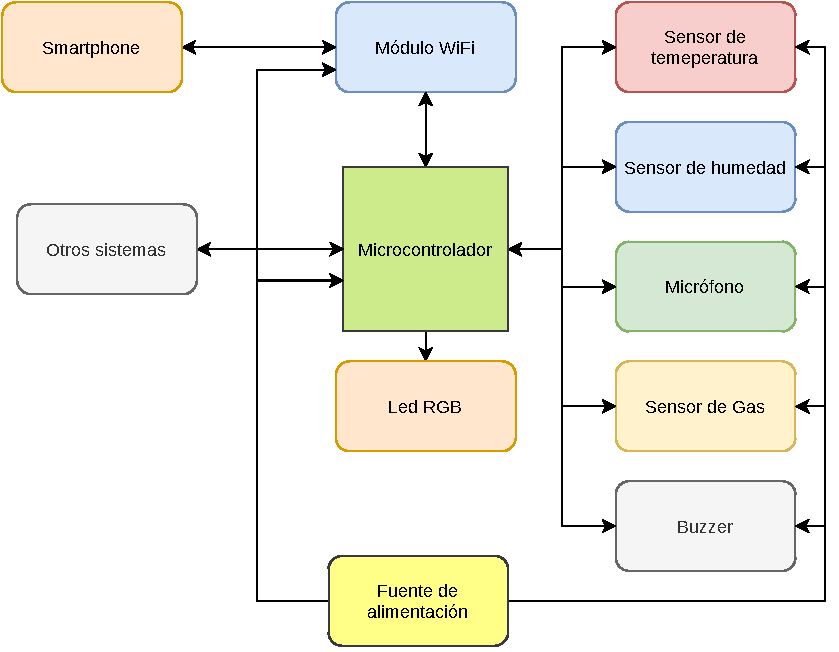
\includegraphics[scale=0.8]{Figuras/bloques.pdf} 
\caption{Diagrama en bloques del analizador modular de ambiente.}
\end{figure}

\section{Pruebas de sistema}
Estas pruebas aseguran el cumplimiento de los requerimientos del proyecto, en este caso se definen siete ensayos para el componente "Adquisición de datos provenientes de sensores" del analizador modular de ambiente.
\\ A continuación se detallan los requerimientos del componente tomados del documento de Especificaciones de Requerimientos de Software de la asignatura Ingeniería de Software.\\

\newpage
\vspace{2cm}
\textit{El software deberá comunicarse con un sensor de humedad y temperatura HTU21D mediante protocolo de comunicación I2C.
[SW-AM-ER-0001-REQ0001]}
\vspace{2cm}
\\ \textbf{NOTA:} un algoritmo realizará la simulación de la respuesta del sensor para comprobar los casos de prueba de desbordamiento en los valores leidos para la temperatura como la humedad.
\vspace{2cm}
\\Los requerimientos a testear se definen a continuación:
\begin{itemize}
\item 1. Al iniciar el sistema, el software deberá inicializar la comunicación I2C para comunicarse con el sensor de humedad y temperatura HTU21D. La función init deberá retornar \textit{INIT\_ I2C\_ OK }. 
\item 2. Si el sensor está desconectado, el software deberá hacer parpadear un led de fallo con una frecuencia  definida, en este caso, dos veces por segundo,  y deberá indicar al usuario, mediante la APP que el sensor no se encuentra conectado.
\item 3. El software realiza consultas periódicas de los valores de temperatura y humedad, luego convierte los datos a grados celcius y la humedad en porcentaje. En caso de error en la lecutura, la función deberá retornar 0xFF.
\item 4. Con el algoritmo de test para desbordamiento, generar una respuesta del valor de temperatura que esté por debajo de -40°C y por encima de 125°C y verificar que la función de lectura retorne 0xFF.
\item 5. Verificación y constatación del valor de temperatura leida (variable TEMP) con el valor real medido con un termómetro auxiliar. El valor leido debe ser igual al valor indicado por el termómetro auxiliar (resolución +/- 1°C). Si existe una diferencia mayor de +/-1°C se debe calibrar el sensor y repetir el caso de prueba. En caso de error en la lecutura, la función deberá retornar 0xFF.
\item 6. Con el algoritmo de test para desbordamiento, generar una respuesta del valor de humedad en \% que esté por debajo de 0 y por encima de 100 y verificar que la función de lectura retorne 0xFF.
\item 7. Verificación y contrastación de la humedad leida (variable HUM) con el valor real medido con un Higrómetro con una tolerancia de +/- 5\%. En caso de poseer una diferencia mayor, se deberá calibrar el sensor y repetir el caso de prueba. Si el valor leido está fuera del rango que indica el fabricante (0 -100), la función deberá retornar 0xFF indicando que hubo un error en el dato leido.
\end{itemize}

En la siguiente tabla, se resumen los casos de pruebas mencionados anteriormente:


\FloatBarrier
\begin{table}[!ht]
    \centering
    \begin{tabularx}{\linewidth}{@{}|c|X|c|@{}}\hline \hline
        \rowcolor[HTML]{d6c6c3}
 CASO & CONDICIÓN & SALIDA \\ 
        \hline     
      1 & I2C INICIALIZAR & \textit{INIT\_ I2C\_ OK }.  \\ 
        \hline
      2  & I2C INICIALIZAR & \textit{INIT\_ I2C\_ NOK }.  \\   
       \hline
      3 & SENSOR CONECTADO & \textit{COM\_ HTU21D\_ OK }.  \\
        \hline
      4 & SENSOR DESCONECTADO & \textit{COM\_ HTU21D\_ OK }, \textit{BLINK\_ LED\_ ERROR(2Hz) }\\
        \hline
      5 &TEMPERATURA < -45°C& \textit{0XFF}\\ 
        \hline
        6 &TEMPERATURA > 125°C& \textit{0XFF}\\ 
        \hline
        7 &-45°C < TEMPERATURA < 125°C& \textit{TEMP}\\ 
        \hline
         8 &HUMEDAD > 100\% & \textit{0XFF}\\ 
        \hline
         9 &HUMEDAD < 0\% & \textit{0XFF}\\ 
        \hline
         10 &0\% < HUMEDAD < 100\%& \textit{HUM}\\ 
          \hline
    \end{tabularx}
    \caption{Casos de pruebas.}
\end{table}
A continuación se observa el árbol con los casos de pruebas:
\FloatBarrier
\begin{figure}[!ht]
 \centering
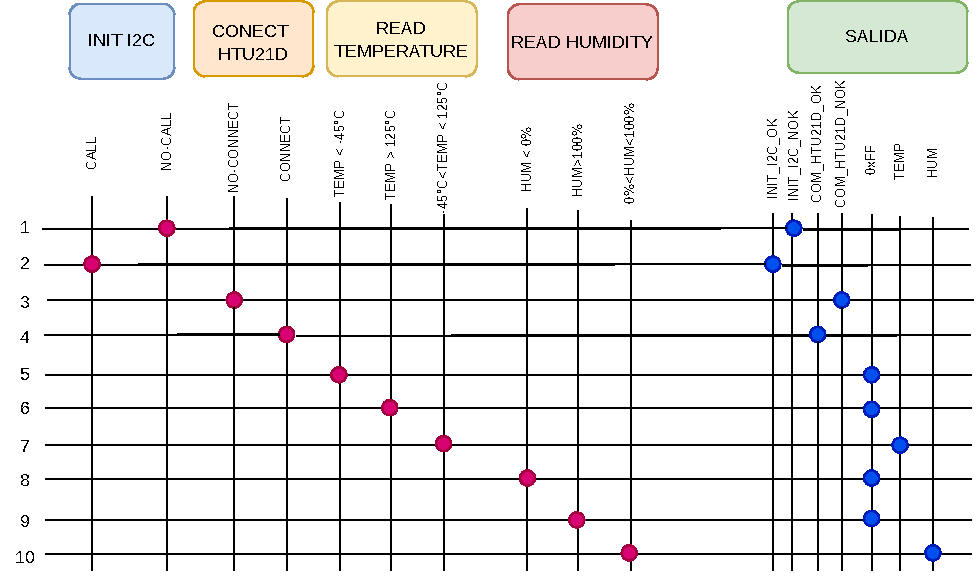
\includegraphics[scale=1]{Figuras/casos.pdf} 
\caption{Árbol de casos de pruebas.}
\end{figure}
\section{Pruebas de aceptación}
Las siguientes pruebas de aceptación se realizarán sobre el prototipo funcionando en un hogar.
\begin{itemize}
\item Prueba 1: realizada la configuración de conexión del módulo con la APP, se verifica el valor de la temperatura observada en la pantalla del smartphone y se compara con un termómetro digital de contrastación.
\item Prueba 2: se desconecta sensor de temperatura y humedad, se verifica que en la APP se visualice el mensaje de sensor desconectado.
\end{itemize}
\end{document}